\setlength{\parindent}{4ex}
\setlength{\parskip}{1ex}

\section{Architectural design}

\subsection{Overview}
	\subsubsection{Context viewpoint}
	
		\begin{figure}[h]
			\centering
			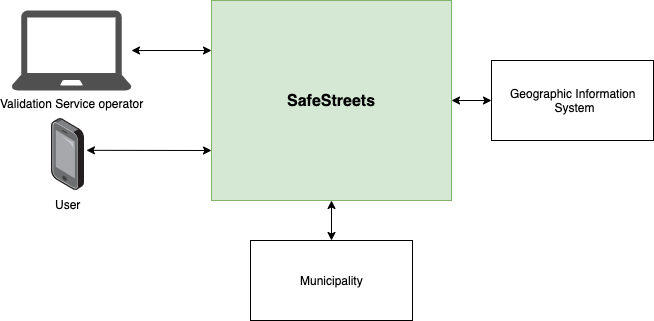
\includegraphics[width=\linewidth]{diagrams/contextViewPoints.png}
			\caption{
				\label{fig:contextViewPoint} 
				Context viewpoint
			}
		\end{figure}

		The system will interact with three actors: users, the Municipality and the Geographic Information System.
		Moreover we recognize that in most of the interactions the system is providing a service to agents so, after taking in consideration different alternatives, we decided to use a client-server architectural approach.

		\begin{figure}[h]
			\centering
			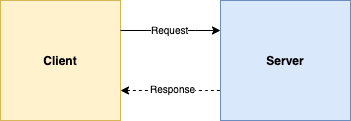
\includegraphics[width=0.5\linewidth]{diagrams/ClientServer.png}
			\caption{
				\label{fig:ClientServer} 
				Client Server architecture
			}
		\end{figure} 
		
	\subsubsection{Composition viewpoint}
	
		\begin{figure}[h]
			\centering
			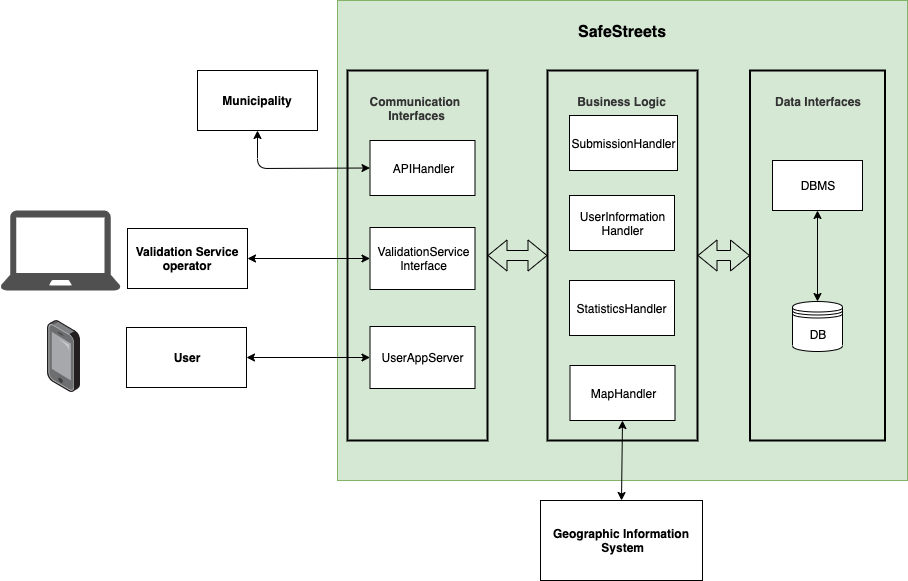
\includegraphics[width=\linewidth]{diagrams/ComponentOverview.png}
			\caption{
				\label{fig:compositionViewPoint} 
				Composition viewpoint
			}
		\end{figure}
		  
		Going deeper in the analysis of our system composition, we are able to identify some of the modules that will be required in order to provide the functionalities specified in the Requirement Analysis and Specification Document. 
		\paragraph{Communication Interfaces}
			Since our system interacts with many external agents, it needs to have different \emph{Communication Interfaces} in order to communicate with them. 
		\begin{itemize}
			\item An API is needed to ensure that the \emph{Municipality System} will be able to share information with our system
			\item A software module is needed in order to support the mobile app that will be offered to the users in order to exploit the functionalities of the system 
			\item A software module is needed to provide the \emph{Customer Care} the functionalities it needs
		\end{itemize}

		\paragraph{Business Logic}
			The actual application logic of our system needs to manage the users information, reports and violations information; for each of these purposes several software modules are necessary; they will use communication interfaces to communicate with the agents and they will be able to retrieve data from the data interfaces.
		\paragraph{Data Interface}
			Our system needs a way to access and store the data it produces or retrieves from external resources, that is why \emph{Data Interface} modules are needed. These modules allows interaction between the \emph{Business Logic} modules and the System Databases; moreover they provide an interface to communicate with the GIS in order to allow the \emph{Business Logic} modules to access its functionalities.

\clearpage

\subsection{Component view}
	\begin{figure}[ht!]
		\centering
		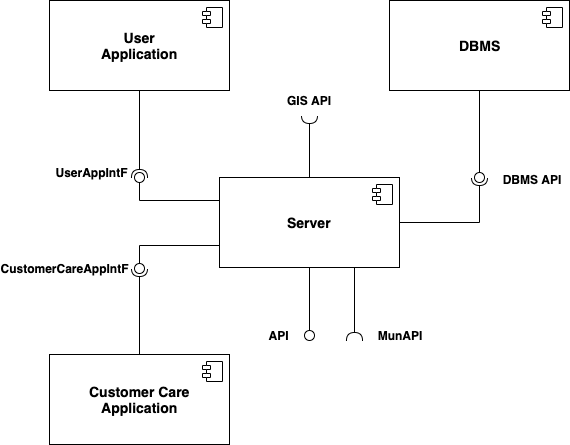
\includegraphics[width=\linewidth]{diagrams/highLevelComponents.png}
		\caption{
			\label{fig:highLevelComponents} 
			High-level components
		}
	\end{figure} Considering all the previous graphs, we have identified the following high level components and interfaces, shown in \autoref{fig:highLevelComponents}, implementing the functionalities defined in the RASD \cite{RASD}:


\begin{itemize}

	\item \textbf{User Application}
	\begin{itemize}
		\item Register
		\item Login
		\item Submit a new violation
		\item View the map with user's own previous submissions
		\item View the map with all the violations by street
		\item View the map with safe and unsafe areas
		\item Consult statistics about violations
		\item View and edit personal information
	\end{itemize}
	\clearpage
	\item \textbf{SafeStreets Operator Application}
	\begin{itemize}
		\item View each user profile, including personal information, submissions history and violations history
		\item Mark and unmark users as banned
		\item Analyse and approve (or reject) violation reports
	\end{itemize}
	
	\item \textbf{DBMS}
	\begin{itemize}
		\item Store and retrieve data
	\end{itemize}	
	
	\item \textbf{GIS API}
	\begin{itemize}
		\item Retrieve a reference to an up-to-date map
		\item Enrich the map with the requested violations
		\item Enrich the map with graphics representing safe and unsafe areas
	\end{itemize}
	
	\item \textbf{Municipality API}
	\begin{itemize}
		\item Retrieve information about accidents
	\end{itemize}
	
	\item \textbf{API}
	\begin{itemize}
		\item Expose information about the submitted violations
		\item Suggest possible solutions to avoid violations
	\end{itemize}
\end{itemize}
\clearpage

\subsubsection{DB component}
\paragraph{ER model}In \autoref{fig:ERModel} is represented the ER model of the system's database.

\begin{figure}[h!]
	\hspace*{-0.7cm}
	\centering
	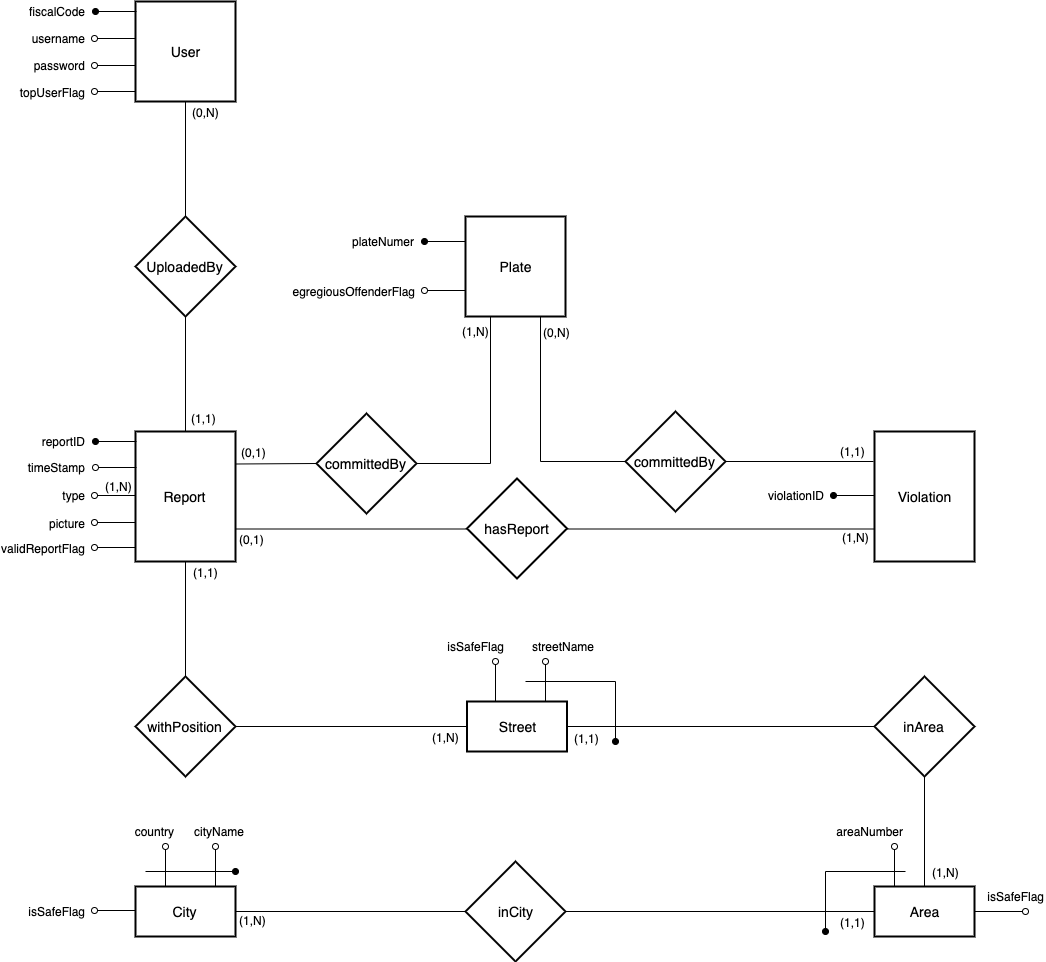
\includegraphics[width=1.1\linewidth]{diagrams/DBComponent.png}
	\caption{
		\label{fig:ERModel} 
		ER model
	}
\end{figure}

\paragraph{Users} Beyond the primary key, the \mbox{\emph{username}} of each registered user must be unique.

\paragraph{Reports}
Reports are identified by a unique \emph{reportID}, but also the couple \\ \emph{(uploadedBy,timeStamp)} must be unique. Every report can have one or more types; the committedBy Plate represents the manual inserted plate number, so it's an optional value.
The \emph{hasViolation} field can be empty until the report is validated and approved, so it's used in pair with the \emph{validReportFlag}, which is also optional in order to distinguish between validated and to be validated reports.

\paragraph{Violations}Beyond the primary key, the \mbox{\emph{hasReport}} attribute must be unique. The \mbox{\emph{committedBy}} field is set to the recognised and validated Plate.

\paragraph{Plates} Every plate is identified by its number; the \emph{egregiousOffenderFlag} is used to indicate whether the owner of the vehicle having that plate often commits violations.

\paragraph{Streets} Every street is identified by the couple \emph{(streetName,area)} which must be unique. The \emph{isSafeFlag} represents whether there are enough violations that took place in that street in order to mark it as unsafe.

\paragraph{Areas} An area is identified by the couple \emph{(areaName,city)} which must be unique. The \emph{isSafeFlag} represents whether there are enough violations that took place in that area in order to mark it as unsafe.

\paragraph{Cities} A city is identified by the couple \emph{(cityName,country)} which must be unique. The \emph{isSafeFlag} represents whether there are enough violations that took place in that city in order to mark it as unsafe.
\clearpage
\subsubsection{Server component}
In this section, we illustrate the \emph{Server} structure and its main components and interactions, in order to explain how interfaces, communication with external components and system functionalities are performed and managed.
\\

The white box representation (\autoref{fig:ServerComponent}) shows the parts composing the \emph{Server} component and their interactions by means of lollipop-socket notation. When designing this component's internal structure, several concerns and requirements were taken into account:
\begin{itemize}
	\item All of its required and provided interfaces had to be delegated to some part of its internal structure
	\item All of the functionalities related to violation submission and report validation had to be addressed and provided by some parts of this component
	\item Interface specific parts had to be designed in order to communicate in different ways with different external components
	\item Associations between internal components needed to be clarified
\end{itemize}

\begin{figure}[h]
	\centering
	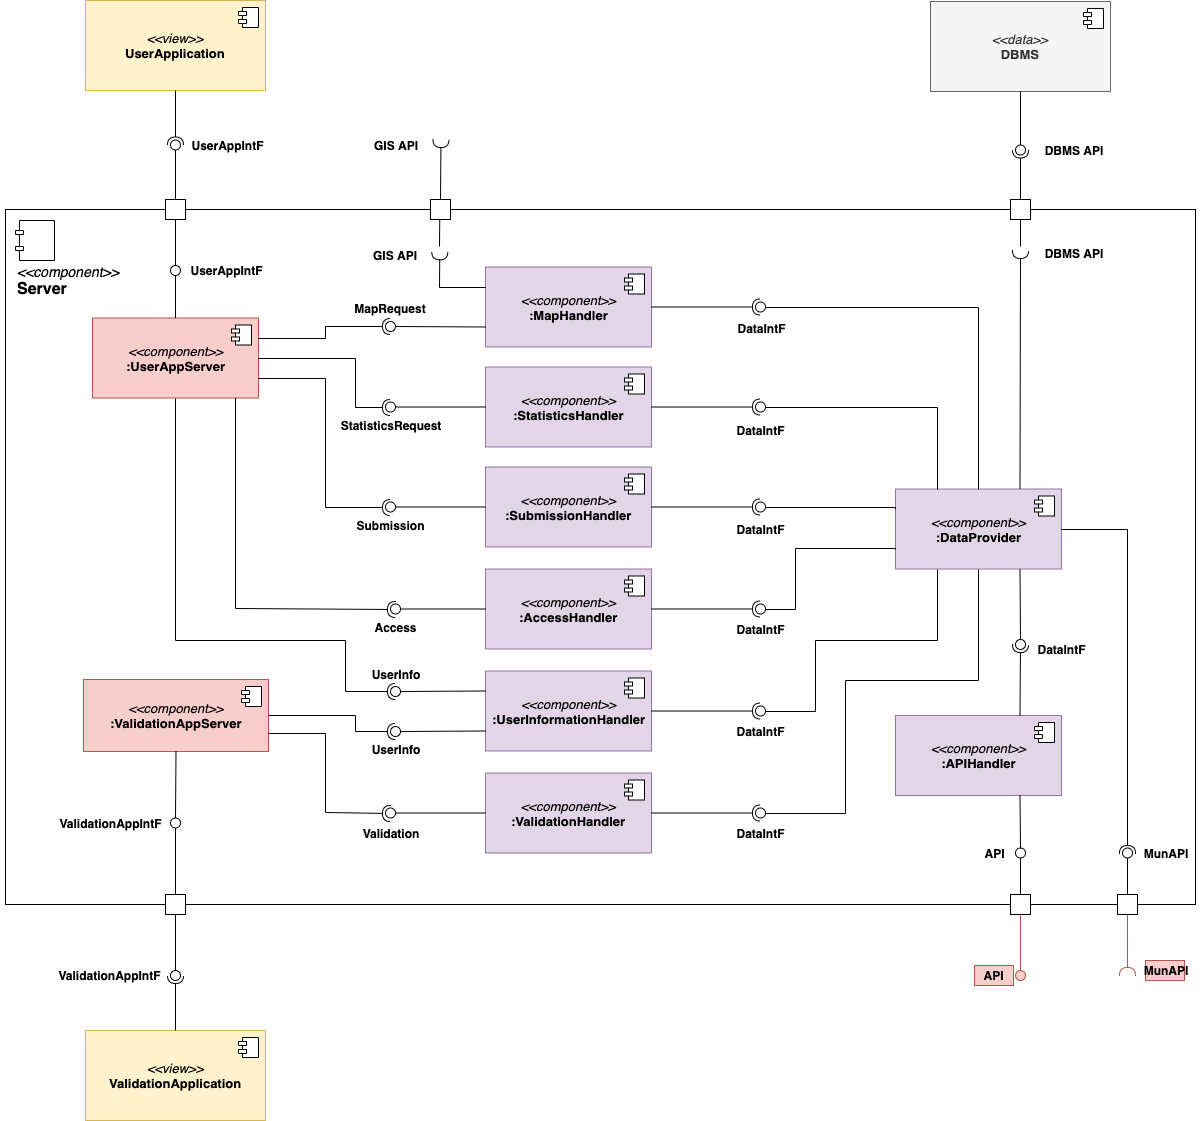
\includegraphics[width=0.95\linewidth]{diagrams/ServerComponent.png}
	\caption{
	\label{fig:ServerComponent} 
		Server component
	}
\end{figure}

\paragraph{UserAppServer}
This component acts as an interface between the user and the application logic of the system: it receives users' violation submission requests or information consultation requests and routes them to the specific handler. This component solves the concerns related to the handling of the requests sent by the users without work loading the rest of the application logic. It also allows the decoupling of the application logic from the presentation logic, which has to be realised in a four tier client-server architecture.
\paragraph{ValidationAppServer}
This component provides the \textit{ValidationApplication} client with the information that the operator needs in order to validate the reports submitted by the users and it finally registers the approval or rejection in the \textit{DBMS}. This component was decoupled from the \textit{UserAppServer} component for its structure, but it offers different functionalities and it is only used and accessible by a specific operator via the client application.
\paragraph{MapHandler}
This component processes the map visualisation requests performed by the users. It is supported by an external \textit{GIS Service} to retrieve and enrich the map with the information requested. Each of its modules is in charge of retrieve the information to visualise and contact the map service, providing the necessary data. This approach allows the decoupling of the presentation logic from the application logic.\newline\newline
\begin{figure}[h!]
	\centering
	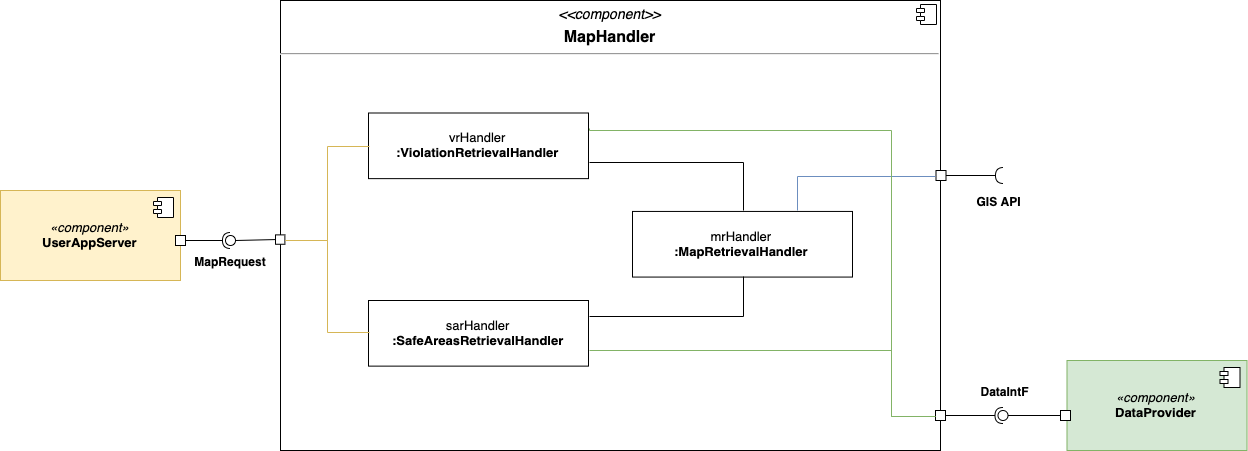
\includegraphics[width=\linewidth]{diagrams/MapHandlerComponent.png}
	\caption{
		\label{fig:mapHandlerComponentDiagram} 
		\emph{MapHandler} object diagram
	}
\end{figure}
\paragraph{StatisticsHandler}
This component processes the statistics requests performed by the users, retrieving data from the \textit{DBMS}, analysing it and turning it into the requested information, which can regard a general or more specific scope. Having a component for this specific purpose enhances decoupling in the system and provides a security layer for the integrity of the data.
\clearpage\paragraph{SubmissionHandler}
This component processes the violation data submitted by the users and the \textit{ImageAnalyser} module is involved to perform the recognition of the license plate in the picture. Finally, the \textit{PlateValidator} module checks whether the recognised plate and possibly the manually inserted plate match and are valid. This data is stored as a report and later validated by the operator to eventually turn it into a violation.\newline\newline
\begin{figure}[h!]
	\centering
	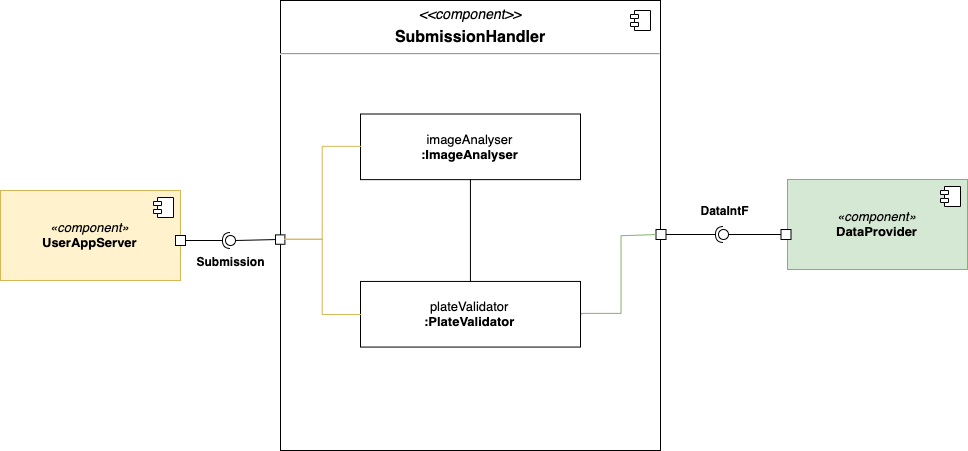
\includegraphics[width=\linewidth]{diagrams/SubmissionHandlerComponent.png}
	\caption{
		\label{fig:submissionHandlerComponentDiagram} 
		\emph{SubmissionHandler} object diagram
	}
\end{figure}
\paragraph{AccessHandler}
This component manages the registration and login phase of the users, encapsulating the logic required to verify the credentials or register new user's information in the \textit{DBMS}. Having a component for this specific purpose enhances decoupling in the system and ensures that these functionalities will not be generate any changes in other components of the system.\newline\newline
\begin{figure}[h!]
	\centering
	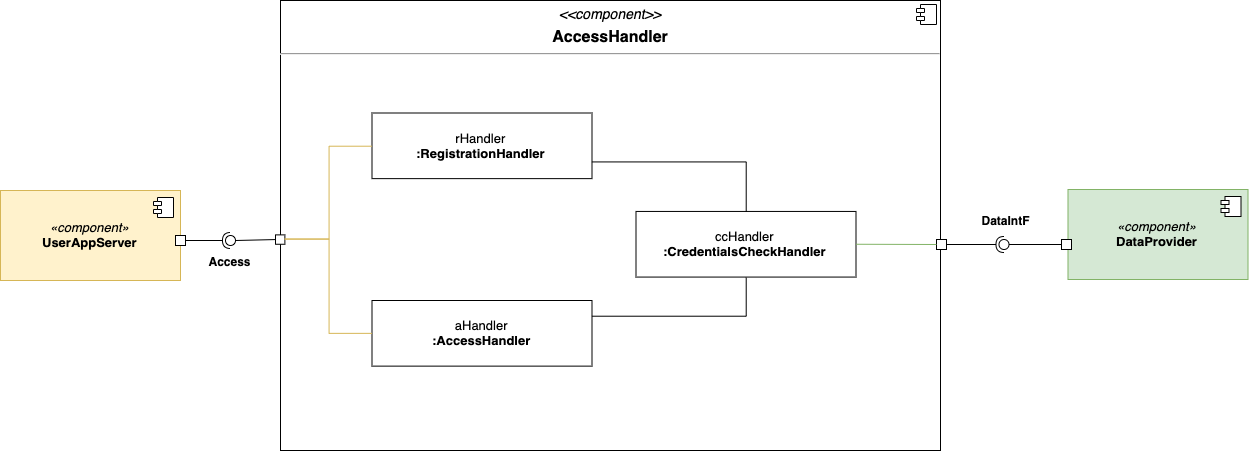
\includegraphics[width=\linewidth]{diagrams/AccessHandlerComponent.png}
	\caption{
		\label{fig:accessHandlerComponentDiagram} 
		\emph{AccessHandler} object diagram
	}
\end{figure}
\paragraph{UserInformationHandler}
This component manages the user information present in the system and provides \textit{UserAppServer} and \textit{ValidationAppServer} the data accessible by the user, given his roles' permissions. The main purpose of this component is to secure users' data, avoiding unauthorised users to consult sensible information. 
\paragraph{ValidationHandler}
This component is used to provide the reports stored in the \textit{DBMS} that still have to be validated to the \textit{ValidationApplication}, in order to allow the \textit{ValidationOperator} to evaluate the submission and decide to approve or reject it. The decision is then stored and the violations information are updated. This component is required to avoid possible malicious or involuntary wrong usages of the system by the customers, trying to submit an unreal violation.
\paragraph{DataProvider}
This component is in charge of providing a unified interface to access the different data sources of the System, both the \textit{DBMS} and the files contained in the File System of the OS hosting the application logic. This component allows a better decoupling between the application logic components and the underlying data layer. \newline\newline\newline

\begin{figure}[h!]
	\centering
	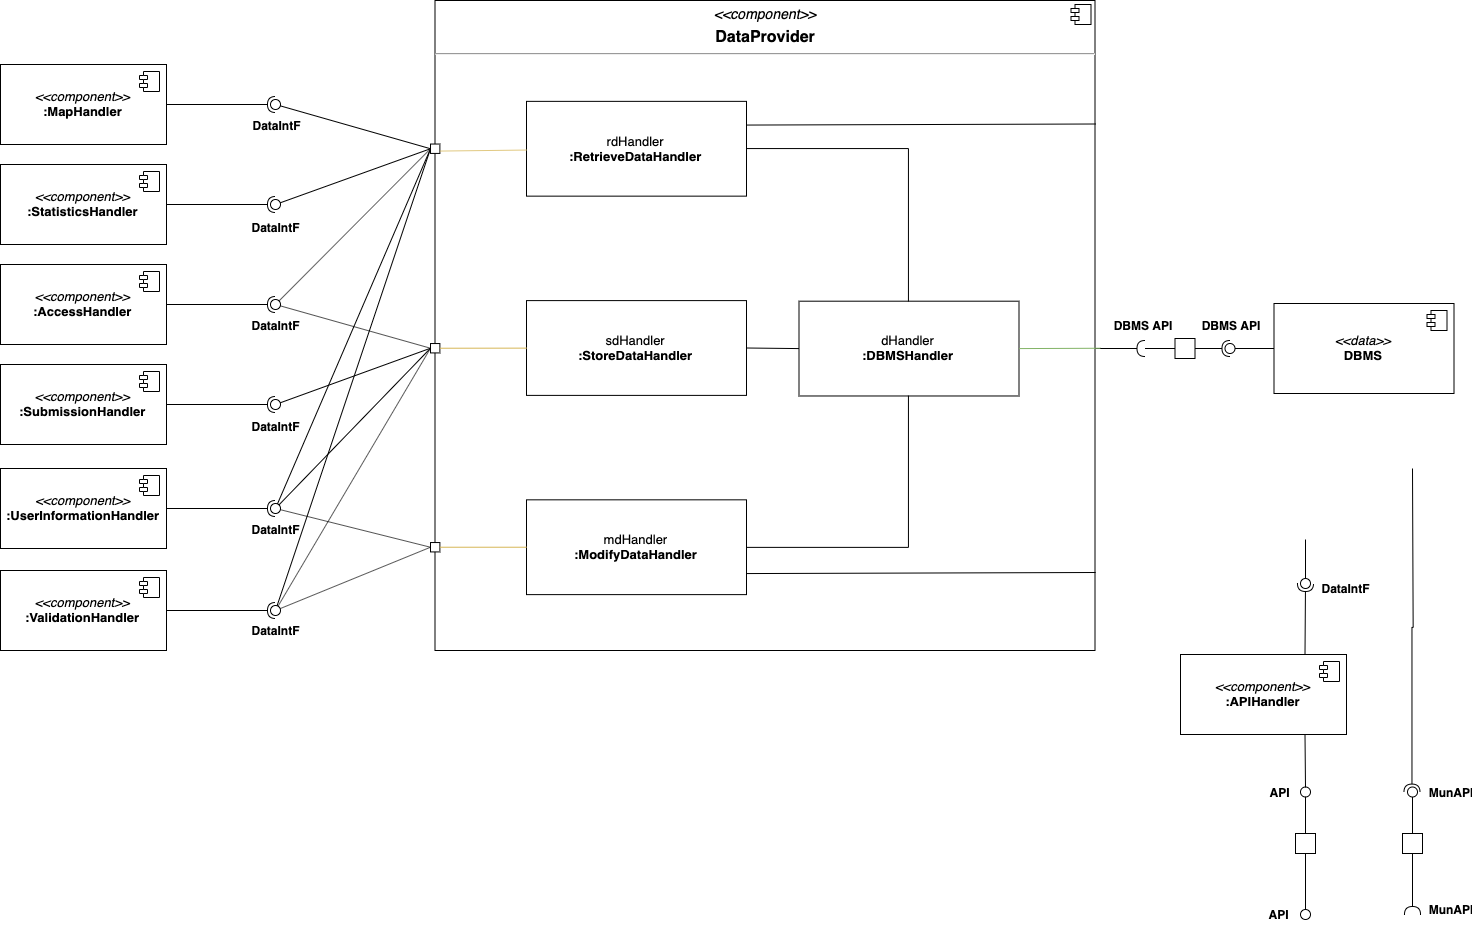
\includegraphics[width=1.1\linewidth]{diagrams/DataProviderComponent.png}
	\caption{
		\label{fig:dataProviderComponentDiagram} 
		\emph{Data Provider} object diagram
	}
\end{figure}

\clearpage

\paragraph{APIHandler}
This component is used to manage the authorities requests of accessing informations about submitted violations. The \textit{SecurityChecker} module guarantees that only authorised municipalities is allowed to retrieve that data. Having a component for this specific purpose enhances decoupling between the presentation layer and the data layer, ensuring data reservation and protection. \autoref{fig:APIHandlerDiagram} shows the internal structure of this component.\newline\newline
\begin{figure}[h!]
	\centering
	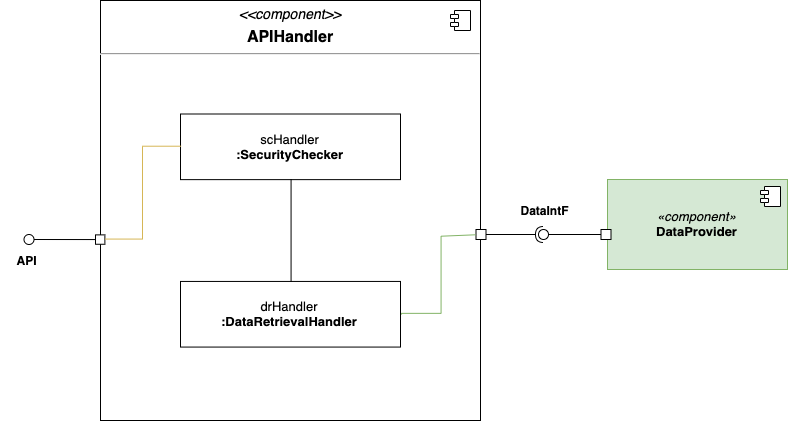
\includegraphics[width=1.1\linewidth]{diagrams/APIHandlerComponent.png}
	\caption{
		\label{fig:APIHandlerDiagram} 
		\emph{APIHandler} object diagram
	}
\end{figure}

\clearpage

\subsection{Deployment view}

\subsubsection{Four tier architecture}
Taking into account that:
\begin{itemize}
	\item the \emph{Composition viewpoint} diagram shows the need of database decoupling from the actual system
	\item in the \emph{Server component view} we can clearly distinguish modules who take care of presentation and communication with the client
	\item in the \emph{Server component view} we can clearly distinguish modules who take care of the specific application logic
\end{itemize}
we decided to design the system on a four tier architecture pattern.\newline\newline

\begin{figure}[h!]
	\centering
	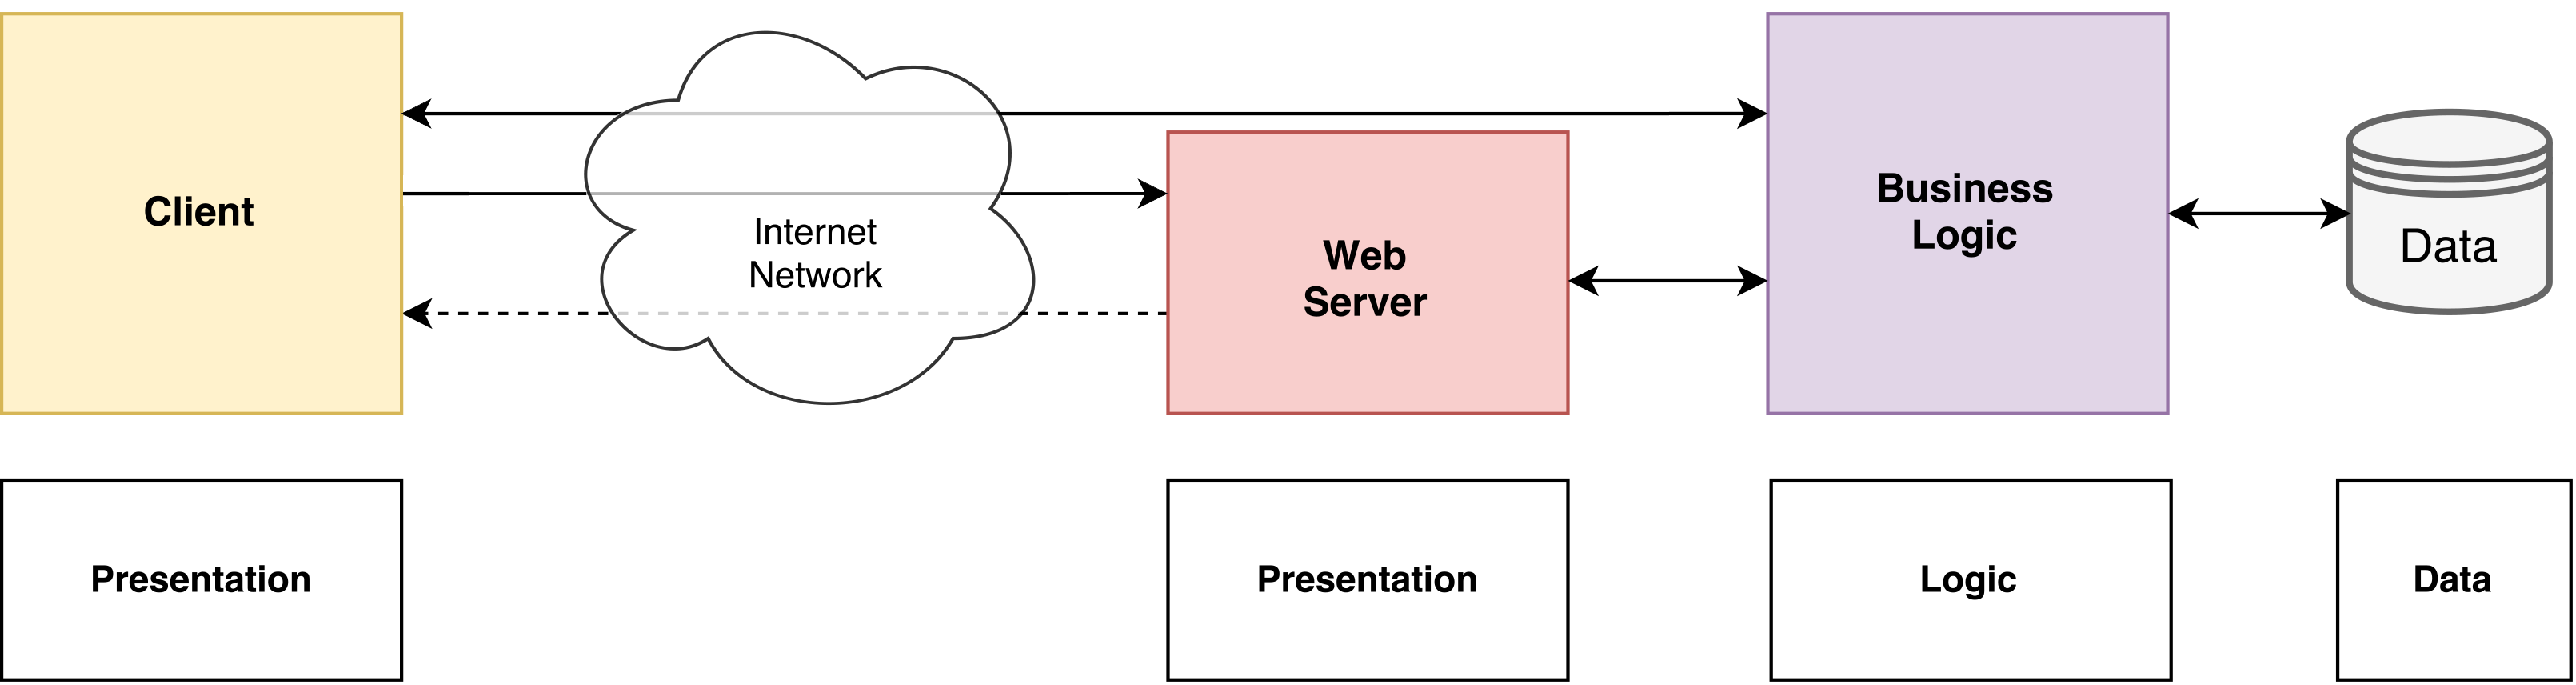
\includegraphics[width=0.9\linewidth]{diagrams/4Tier.png}
	\caption{
		\label{fig:fourTierCloud} 
		Four tier architecture with internet layer
	}
\end{figure}

\paragraph{Mapping of Server components on architecture:}to clarify at a finer level how the Server components are mapped in the four tier layered architecture the following diagram represents the Server components highlighted in the same color of the tier in the previous diagram:
\begin{itemize}
	\item Client: components used by users in order to access the functionalities offered by the system
		\begin{itemize}
			\item UserApplication
			\item ValidationApplication
		\end{itemize}
	\item Web Server: components which provides interfaces to clients in order to allow them to use functionalities offered by the system
		\begin{itemize}
			\item ValidationAppServer
		\end{itemize}
	\item Business Logic: components which realizes the functionalities offered by the system
		\begin{itemize}
			\item UserAppServer
			\item MapHandler
			\item StatisticsHandler
			\item SubmissionHandler
			\item AccessHandler
			\item UserInformationHandler
			\item ValidationHandler
			\item DataProvider
			\item APIHandler
		\end{itemize}
	\item Data: components which store and manage the access to the data produced and needed by the Business Logic
		\begin{itemize}
			\item DBMS \newline\newline
		\end{itemize}
\end{itemize}

\begin{figure}[h]
			\centering
			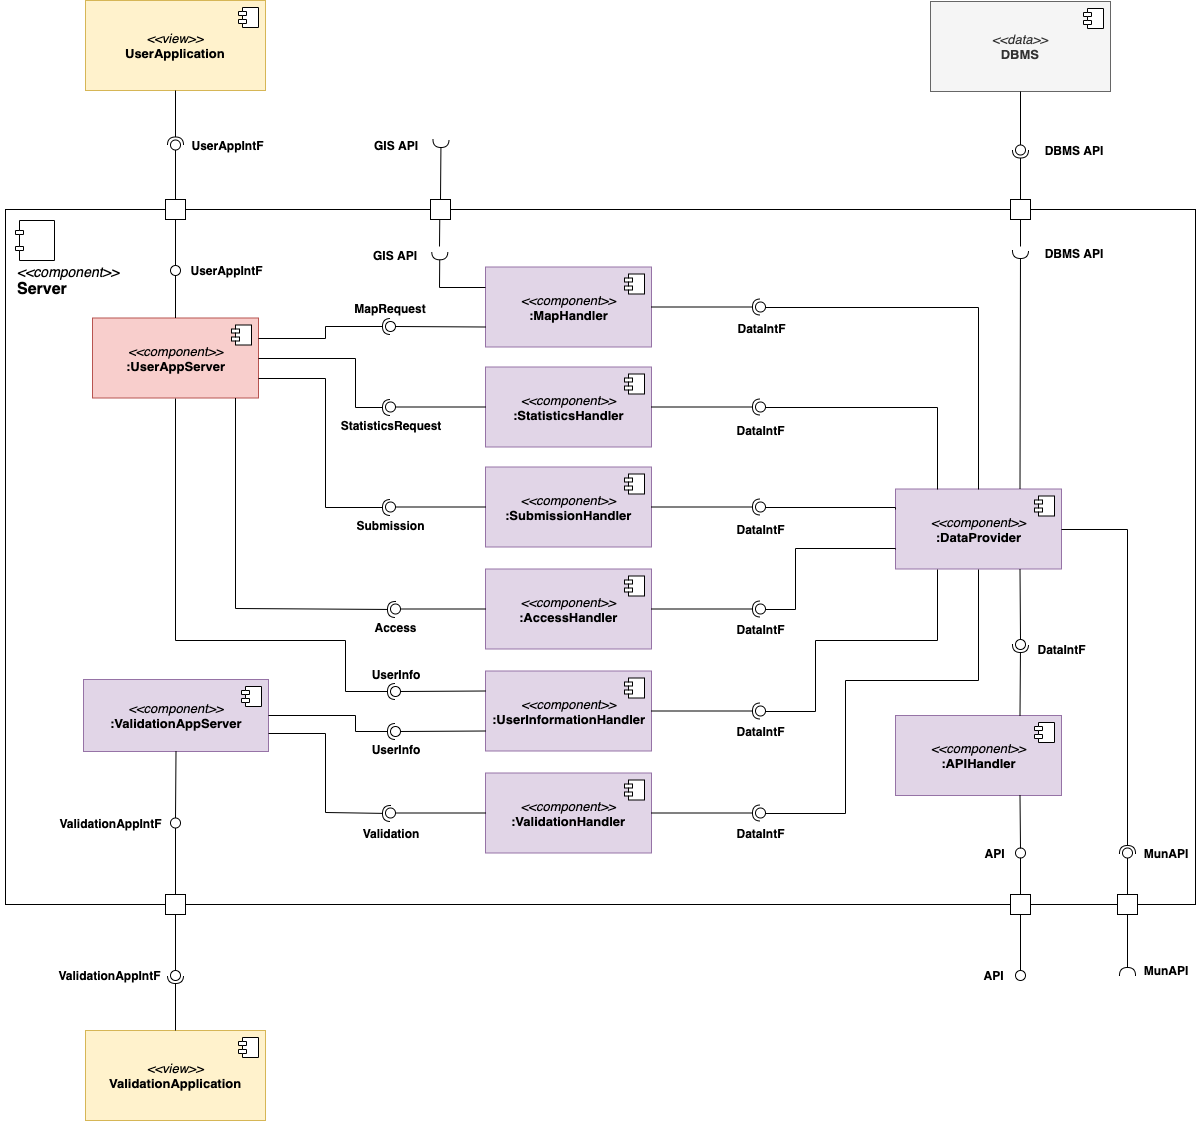
\includegraphics[angle=0,width=0.9685\linewidth]{diagrams/deployComponent.png}
			\caption{
				\label{fig:deployServerComponent} 
				Mapping server component on architecture
			}
		\end{figure}
\clearpage

\label{sec:implementationChoices}
\subsubsection{Implementation choices}
The following technologies were chosen for the implementation of the SafeStreets system. J2EE was the main choice we made because it offers a wide range of functionalities that makes the development of scalable multi tiered web based application much easier than with other technologies.

\paragraph{Web Pages:} JSP was chosen over Servlets because the content of our web pages has few dynamic parts so writing small chunks of Java code in html pages is a more suitable solution
\paragraph{Mobile App:} Java was chosen for server compatibility reasons and in order to deploy the app both on Android and on iOS
\paragraph{Application Logic:} EJB were used to implement the Application Logic components since our application is developed using J2EE
\paragraph{Application Server and Web Server:} GlassFish 5.1 was chosen since it offers containers both for the EJB and the JSP pages 
\paragraph{Provided APIs:} all the API provided by this system are compliant with the REST paradigm so JAX-RS was used
\paragraph{Data - Application Logic Communication:} JPA over JDBC was chosen as a mean to enable communication between the Application Logic and the DBMS.

\paragraph{Web Server - Application Logic Communication:} JNDI was chosen as a naming and directory service to allow the web servers to access the functionalities offered by the Application Logic
\paragraph{DBMS:} MySQL was chosen as DBMS since it is the most popular and widespread and it has a lot of documentation and a big community of users; in combination with it we chose InnoDB which allows the usage of foreign keys
\clearpage
\subsubsection{Decision Tree}
\autoref{fig:decisionTree} represents a summary of the main design and implementation decisions that were made during the development of the architecture of the SafeStreets system.\\

\begin{figure}[h!]
	\centering
	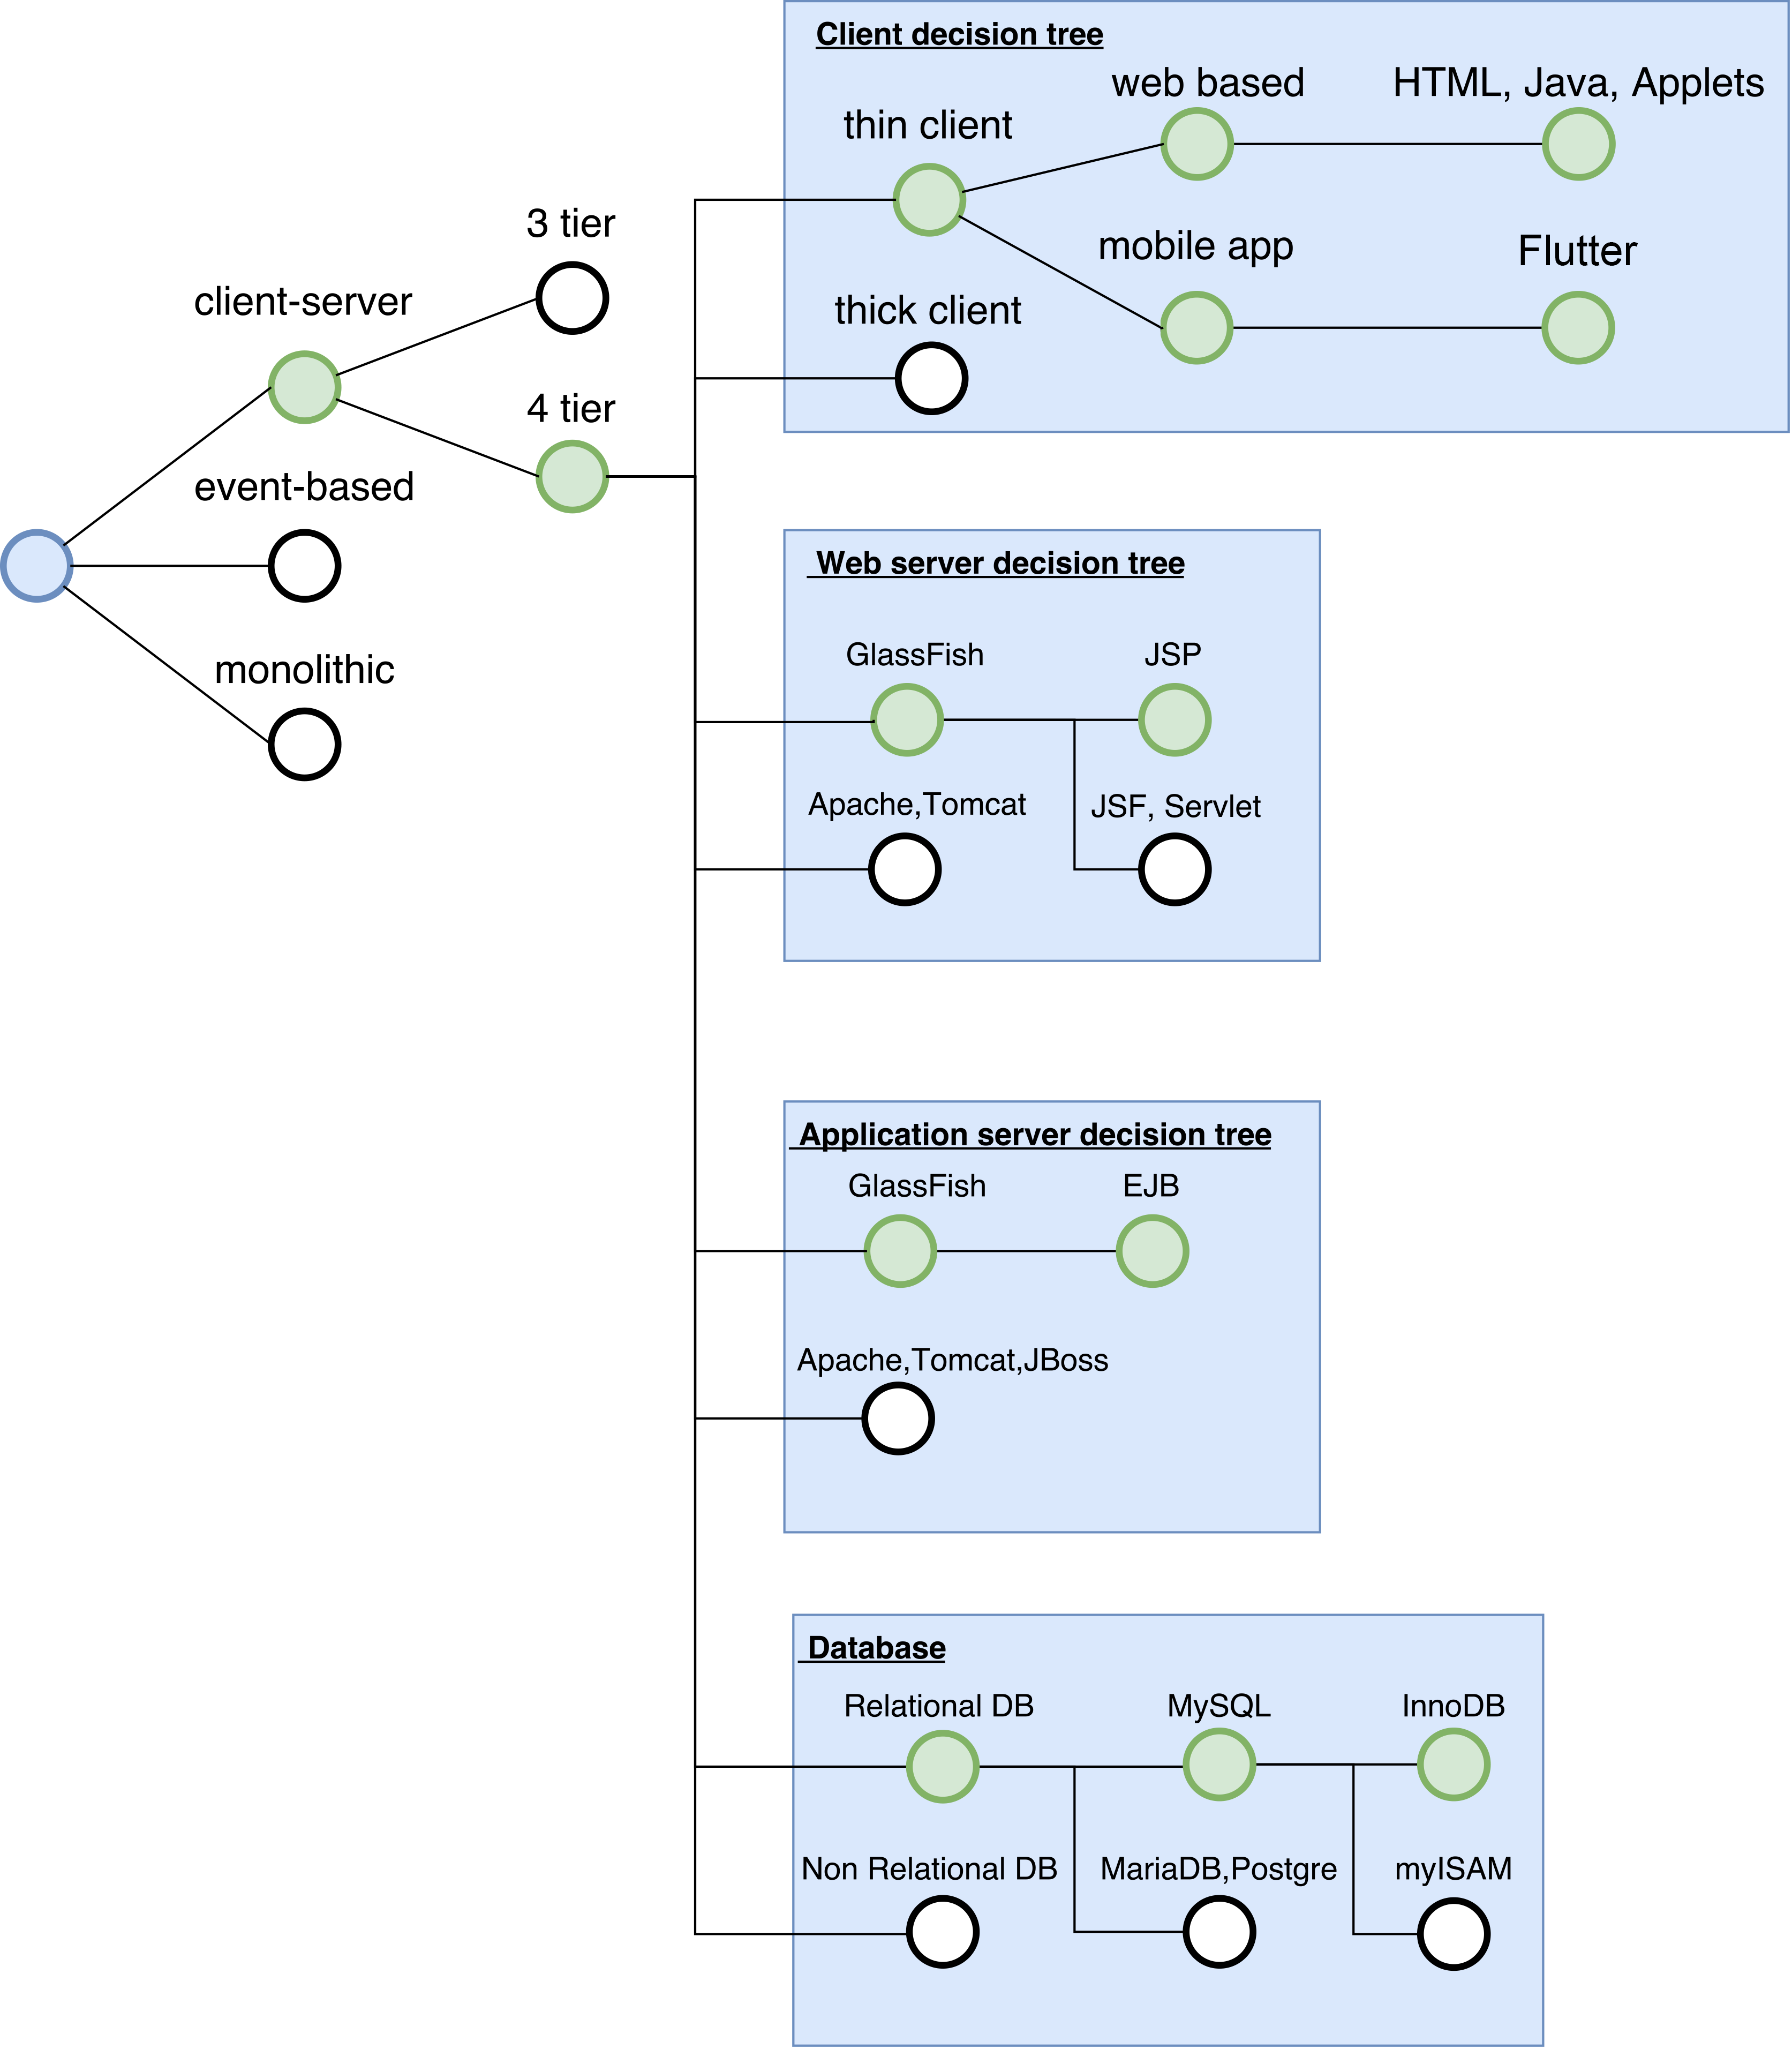
\includegraphics[width=\linewidth]{diagrams/decisionTree.png}
	\caption{
		\label{fig:decisionTree}  
		Decision Tree
	}
\end{figure}
\clearpage
\subsubsection{Deployment diagram} 

The diagram in \autoref{fig:deployment} represents the mapping of the software components depicted in \autoref{fig:deployServerComponent} and \autoref{fig:highLevelComponents} on the devices that will run them. Many design concerns were considered while developing this solution.\newline\newline\newline

\begin{figure}[ht!]
	\centering
	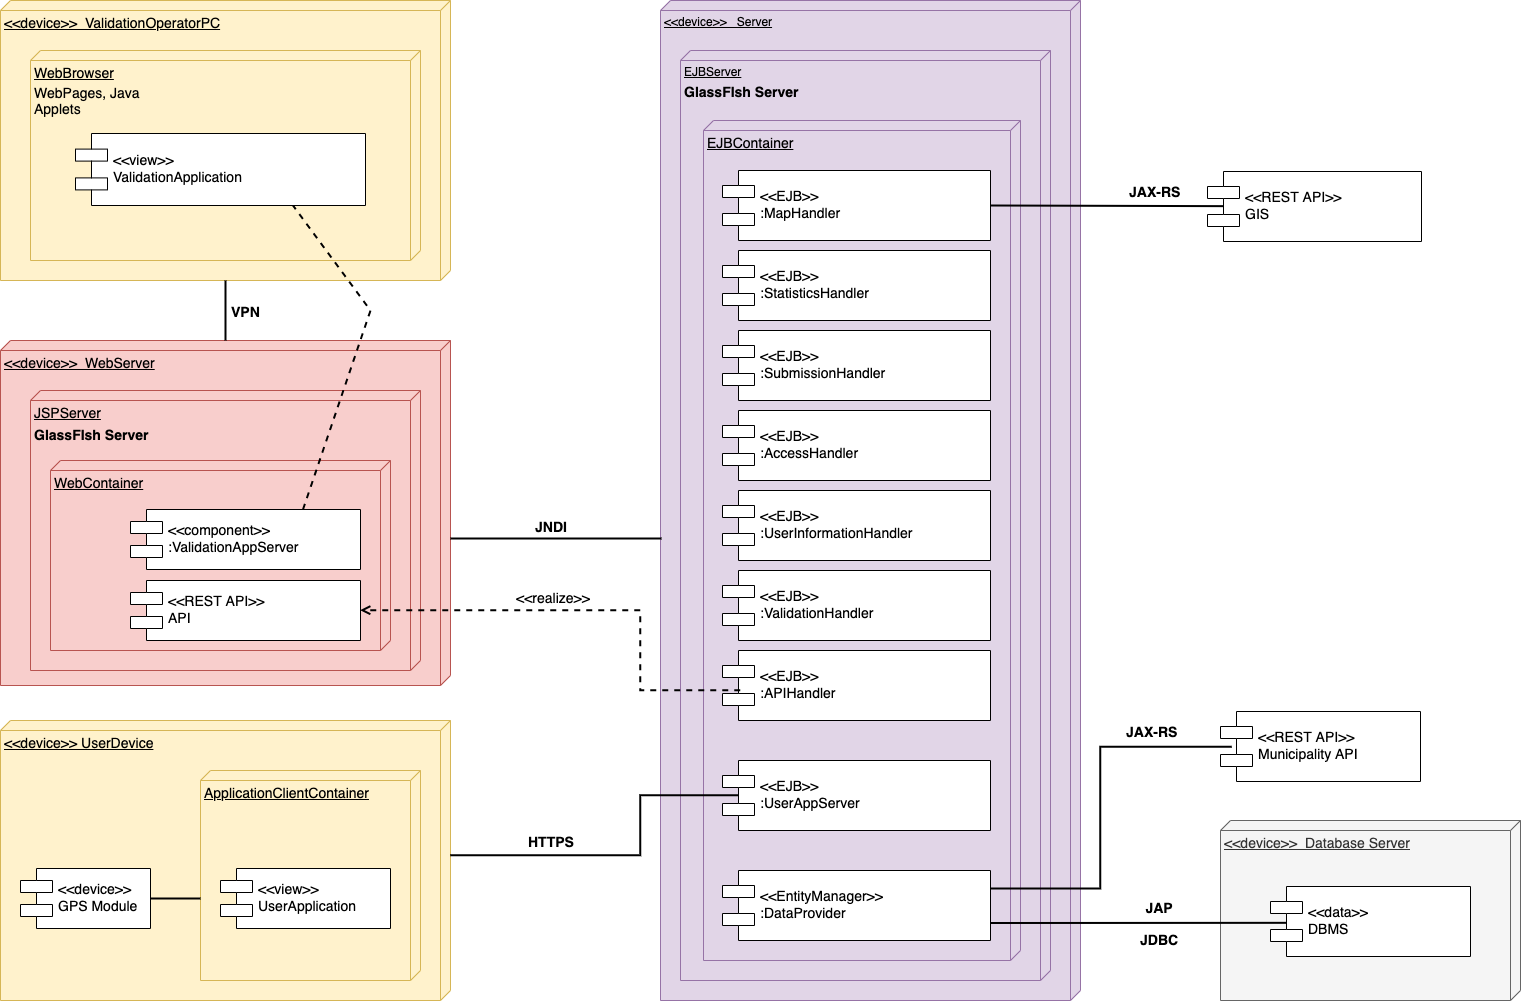
\includegraphics[width=1.2\linewidth]{diagrams/deployment.png}
	\caption{
		\label{fig:deployment} 
		Deployment diagram 
	}
\end{figure}

\clearpage

\paragraph{Security:}security is ensured in different points of the architecture, in particular the \emph{UserAppServer} uses HTTPS as communication protocol to communicate with the users; the devices running the \emph{ValidationApplication} component are in a VPN with the device running the \emph{ValidationAppServer}.
\paragraph{Scalability:}this model of deployment is scalable in the sense that the system administrators will be able to add more devices and deploy more instances of the needed components when and where performance issues will arise, in order to maintain a minimum level of performance even with loads increase.
\paragraph{Decoupling:}decoupling in this architecture is present at different levels; in the deployment diagram it is clear that the each of the four tier runs on different devices, moreover the \emph{UserAppServer} component runs on a different device than the \emph{ValidationAppServer}.
\paragraph{Redundancy:}in this iteration of the architecture no redundancy of components or devices is present, but it is allowed in prevision of future expansions of the system's infrastructure.
\paragraph{Fault Tolerance:}deploying different components on different machines allows the system to be easier to recover in case of a problem on one of the machines; for an example the Web Server running the \textit{ValidationAppServer} component goes down, it can be replaced with another machine and in the mean time the \textit{ApplicationServer} would still be up and running and still be able to provide the \textit{UserApplication} with its functionalities.

\clearpage
\subsection{Runtime view}
In this section we represent some runtime views of the supposed interactions between the components of the \emph{SafeStreets} system.

\paragraph{Notes to read the diagram} When an attribute is modified in a JPA object the changes are reflected into the
	\emph{DataProviderComponent} in order to keep the database updated. 	The \emph{Login Phase} is represented only in the first diagram in order to show how it will be performed but will no be 
	repeated in every diagram in order to improve readability.

\subsubsection{Upload}

	\label{sec:uploadRunView}
	The sequence diagram in \autoref{fig:uploadSubmission} shows how the upload of a report is handled in the Server component of the system.

	\begin{figure}[h!]
		\centering
		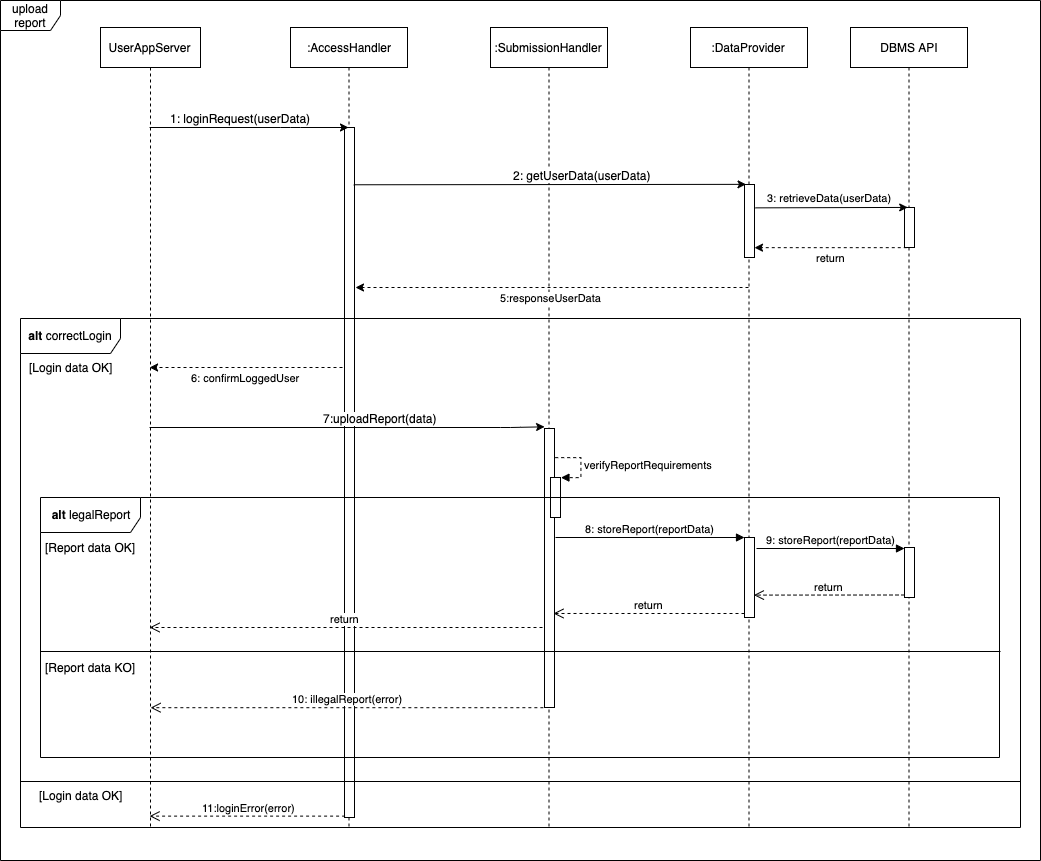
\includegraphics[angle=0,width=\linewidth]{sequence/uploadSubmission.png}
		\caption{
			\label{fig:uploadSubmission} 
			\emph{Upload submission} sequence diagram
		}
	\end{figure}
	\clearpage

\paragraph{Note} As already stated in the following diagrams we will assume that the user has already logged in correctly
	in order to focus on the purpose of the diagram.\\

\subsubsection{Map request}
The sequence diagram in \autoref{fig:mapRequest} shows the map request process.\\

\paragraph{Interactions not represented}
\begin{itemize}
\item The \emph{MapHandler} needs an interaction with the GIS while calling its "processUserDataForMap()" method	
	to process latitude and longitude information needed to generate the right "userData" to query the DBMS. 
\item To improve redeability of the diagram we omitted the interaction between the \emph{DataProvider} and the 
	\emph{Municipality API} since the first checks if the latter has new data regarding the interested area of the 
	map requested before returning data
\end{itemize}

\begin{figure}[h!]  
	\centering
	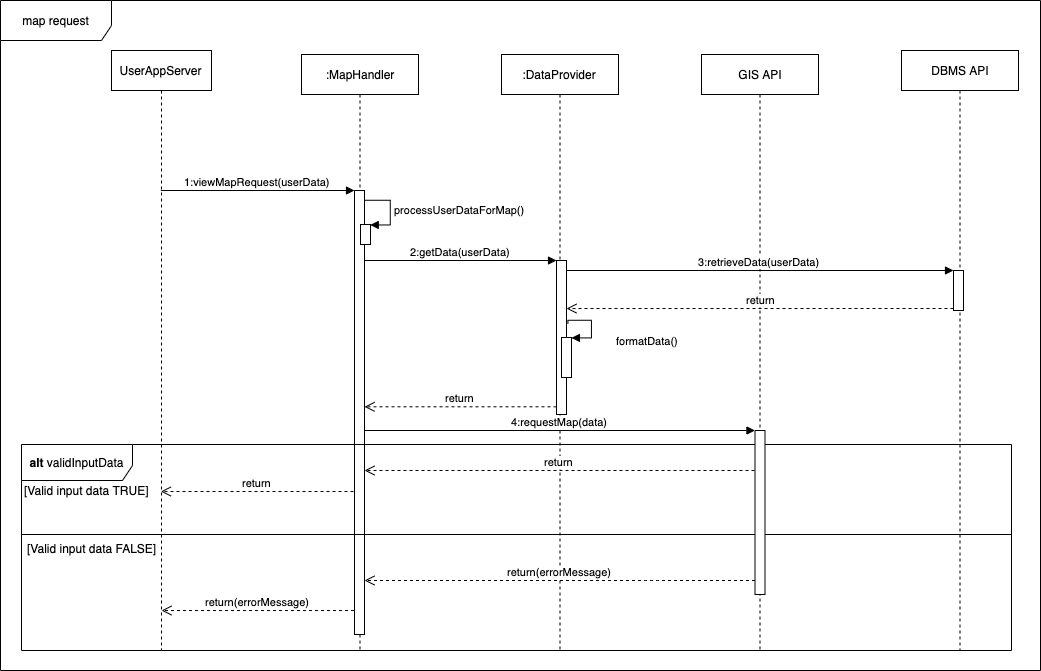
\includegraphics[angle=0,width=\linewidth]{sequence/mapRequest.png}
	\caption{
		\label{fig:mapRequest} 
		\emph{Map request} sequence diagram
	}
\end{figure}

\clearpage
\subsubsection{Show statistic}
The sequence diagram in \autoref{fig:showStatistics} shows the interactions between the modules involved in the process of retrieving data
for a certain statistic and show it to the user.\\

\begin{figure}[h!]
	\centering
	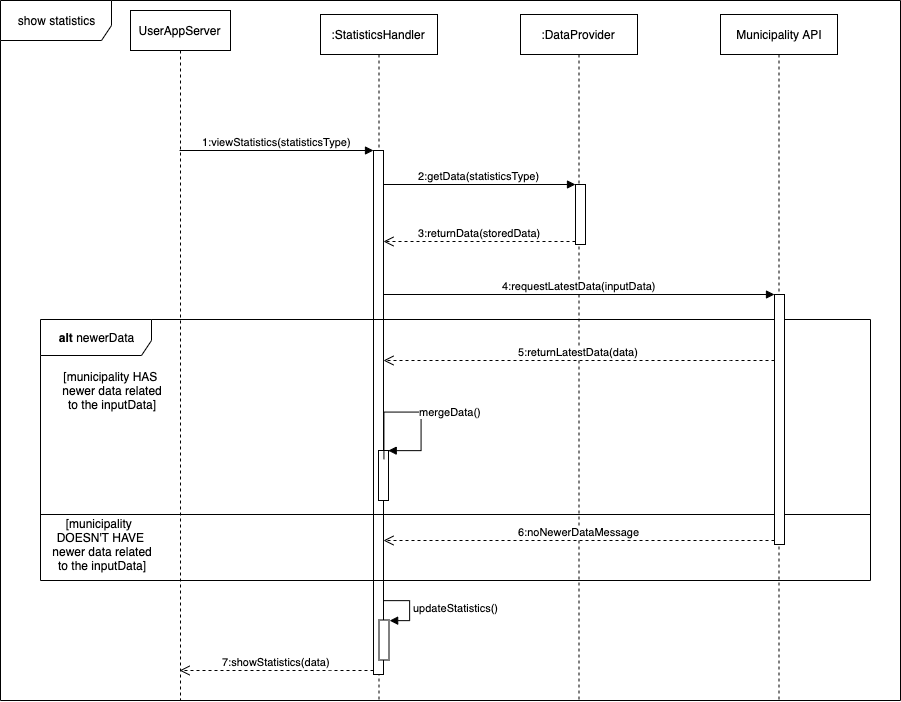
\includegraphics[angle=0,width=\linewidth]{sequence/showStatistics.png}
	\caption{
		\label{fig:showStatistics} 
		\emph{Show statistic} sequence diagram
	}
\end{figure}

\clearpage
\subsubsection{See user info}
The sequence diagram in \autoref{fig:seeUserInfo} shows the interactions between the modules involved in the process of retrieving data of a certain user and show it to the \emph{ValidationApplication}.\\

\begin{figure}[h!]
	\centering
	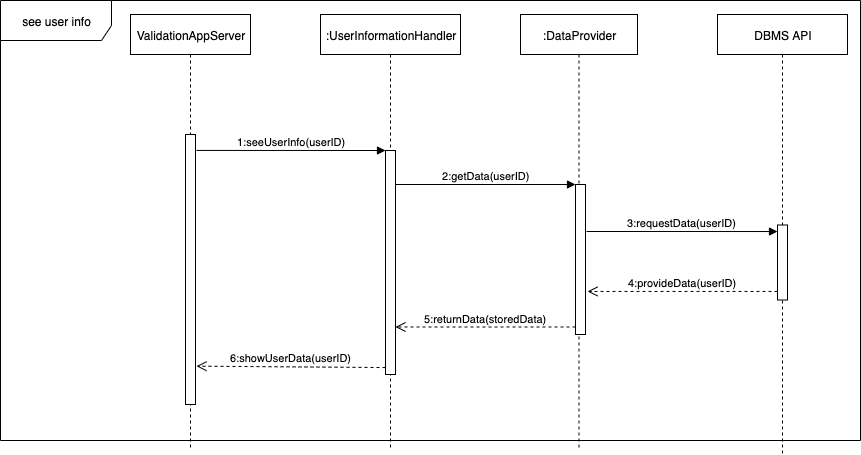
\includegraphics[angle=0,width=\linewidth]{sequence/seeUserInfo.png}
	\caption{
		\label{fig:seeUserInfo} 
		\emph{See user info} sequence diagram
	}
\end{figure}
\clearpage

\subsubsection{Validate reports}
The sequence diagram in \autoref{fig:validateReport} shows the interactions between the modules involved in the process of validating the submitted reports, performed by the \emph{ValidationApplication}.\\

\begin{figure}[h!]
	\centering
	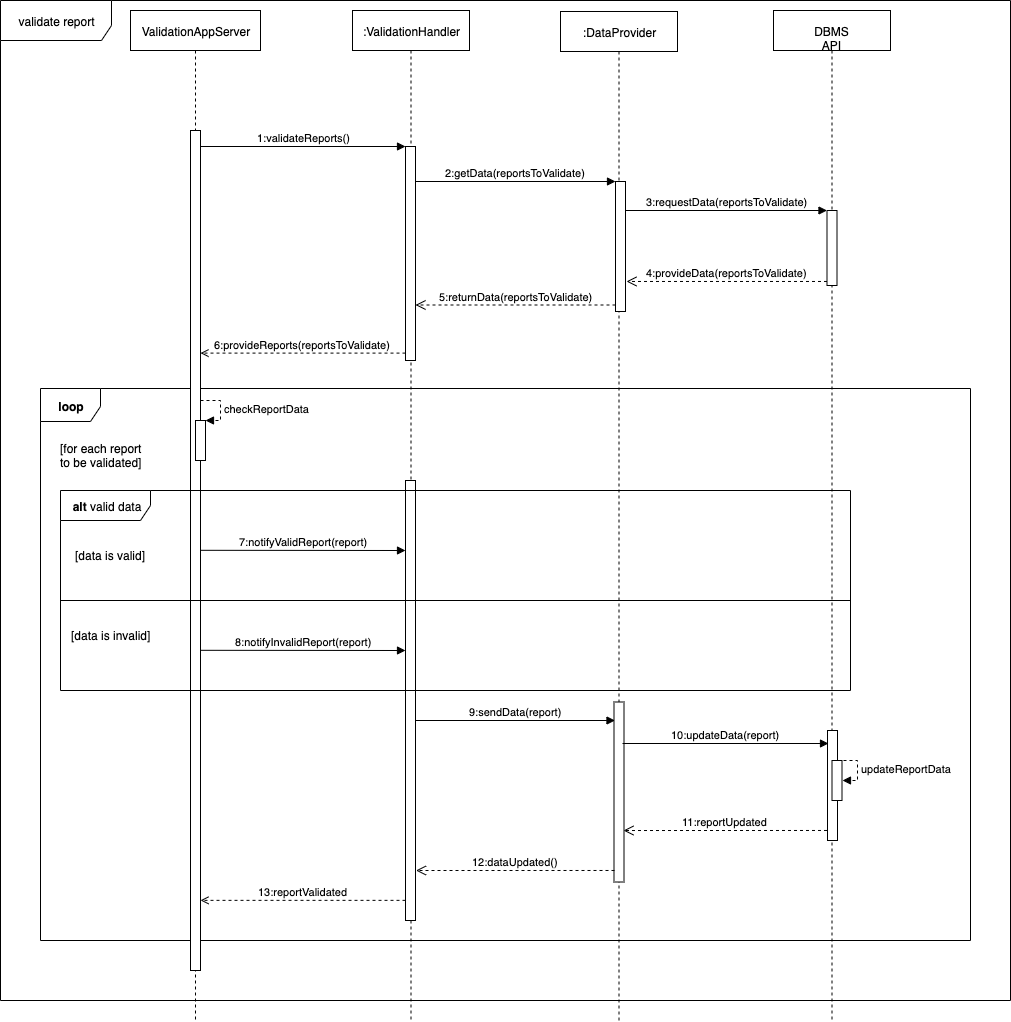
\includegraphics[angle=0,width=\linewidth]{sequence/validateReport.png}
	\caption{
		\label{fig:validateReport} 
		\emph{Validate reports} sequence diagram
	}
\end{figure}
\clearpage

\subsubsection{Send data to municipality}
The sequence diagram in \autoref{fig:sendDataToMun} shows the interactions between the modules involved in the process of providing violations data to the municipality.\\

\begin{figure}[h!]
	\centering
	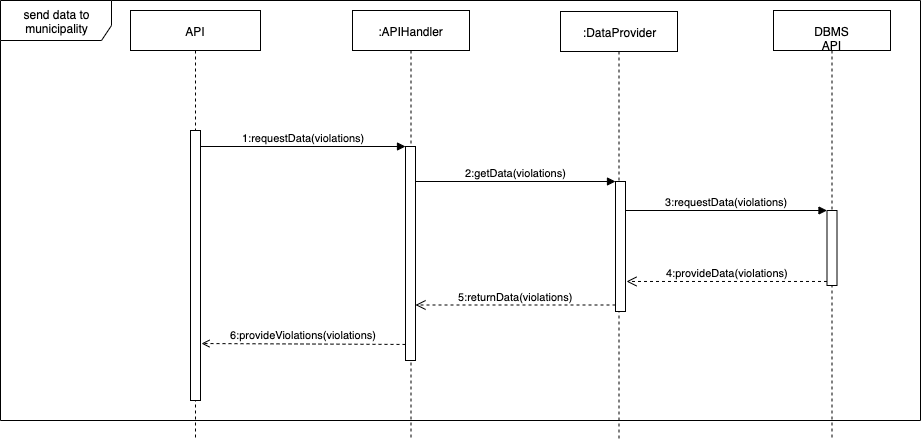
\includegraphics[angle=0,width=\linewidth]{sequence/sendDataToMun.png}
	\caption{
		\label{fig:sendDataToMun} 
		\emph{Send data to municipality} sequence diagram
	}
\end{figure}
\clearpage


\subsection{Component Interfaces}
The component interfaces offered by the application server are represented in the following component interfaces diagram.
The arrows represents the dependencies relations. All the data parameters and return values are classes that implements the JsonValue interface, in order to be optimized for serialization.\\


\begin{figure}[h!]
	\centering
	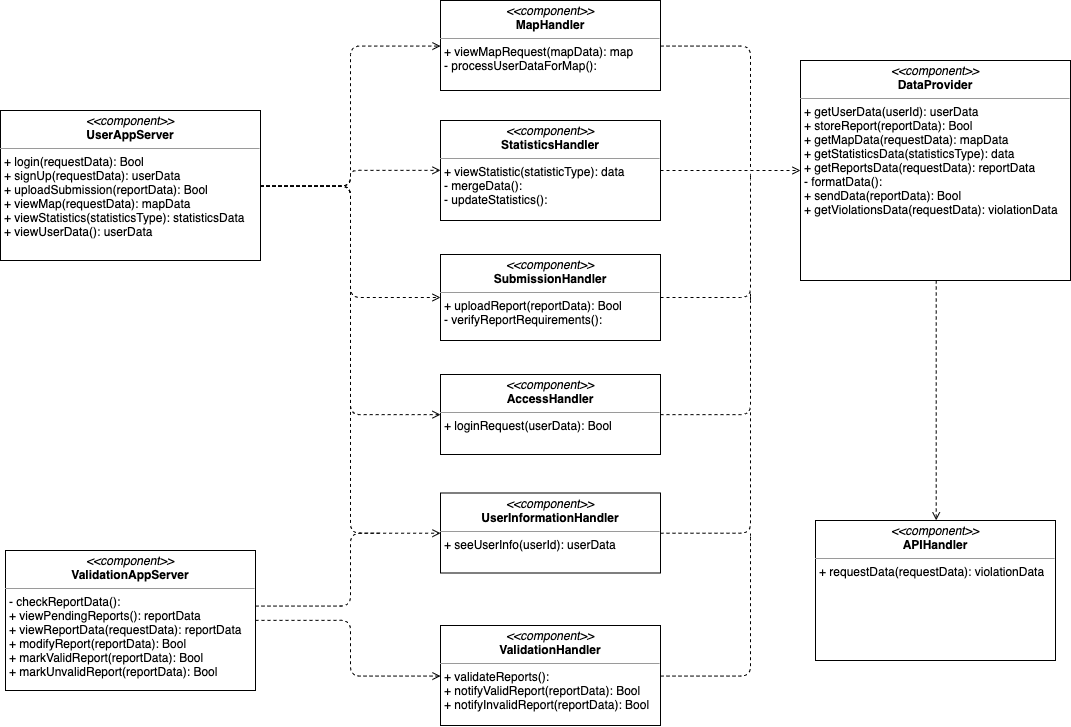
\includegraphics[angle=0,width=1.1\linewidth]{diagrams/ServerComponent-methods.png}
	\caption{
		\label{fig:sendDataToMun} 
		\emph{Component interfaces} diagram
	}
\end{figure}

\subsubsection{User Application interface}
The User Application interface is responsible for communications between the user application and the user application server.
Because of the nature of exchanged data (password and privacy-related information), the protocol to be used is HTTPS.

\subsubsection{Validation Service interface}
Via the Validation Service interface is responsible for communications between the validation service application and the validation application server.

All computers used by the validation service are connected in the same dedicated subnet as the validation application server and this web server is accessible only from the aforementioned subnet. 

A VPN is used to achieve what mentioned above. Because of the sensitive data exchange, the protocol to be used is HTTPS

\subsubsection{Data Provider interface}
Trough the Data Provider API the system can retrieve and write data into the database. Note that the Data Provider component is the only one that access directly the DBMS API component.

\subsubsection{API Handler interface}
The API Handler Interface must be realized using the REST paradigm. The external Municipality system should query the API Handler
in order to retrieve an updated list of violations and statistics. 


